\setRL
\clearpage

\def \MemTB {\Mempath /MembraneTheoreticalBackground}

\section{
چکیده
}
در این فصل با مقدمه‌ای از نقش غشای زیستی در سلول شروع کرده. سپس مروری کوتاهی بر تارخچه‌ی تحقیقات انجام شده در جهت کشف و بررسی ساختار غشای سلول‌های زنده در قرن‌های ۱۹ و ۲۰ میلادی شده‌است. در مورد ساختار واحد‌های تشکیل دهنده‌ی غشا بحث شده و در نهایت در مورد چیدمان غشای هسته یا بسته‌ی هسته توضیح داده شده‌است.

\section{
انحنای غشا
}
\subsection{
تعریف خمش
}

ضخامت غشا از مرتبه‌ی چند نانومتر است و مقیاس انحنا‌هایی که شکل کلی غشا را مشخص می‌کنند از مرتبه‌ی بزرگی میکرون بوده. در نتیجه به طور عمومی مدل کردن شکل و انحنای غشا با یک رویه‌ی ۲ بعدی کاملا قابل قبول است. تصاویر میکروسکوپی غشا مانند شکل‌های 
\ref{fig:budding}
و
\ref{fig:flucmem} 
نشان می‌دهد که غشا سطحی نسبتا صاف و پیوسته دارد. در نتیجه در مقیاس‌های میکرومتری غشا را با رویه‌ای با چنین ویژگی‌ای مدل می‌کنیم. البته که این فرض در مقیاس نانومتری پابرجا نیست. 

\begin{figure}[t]
\begin{center}
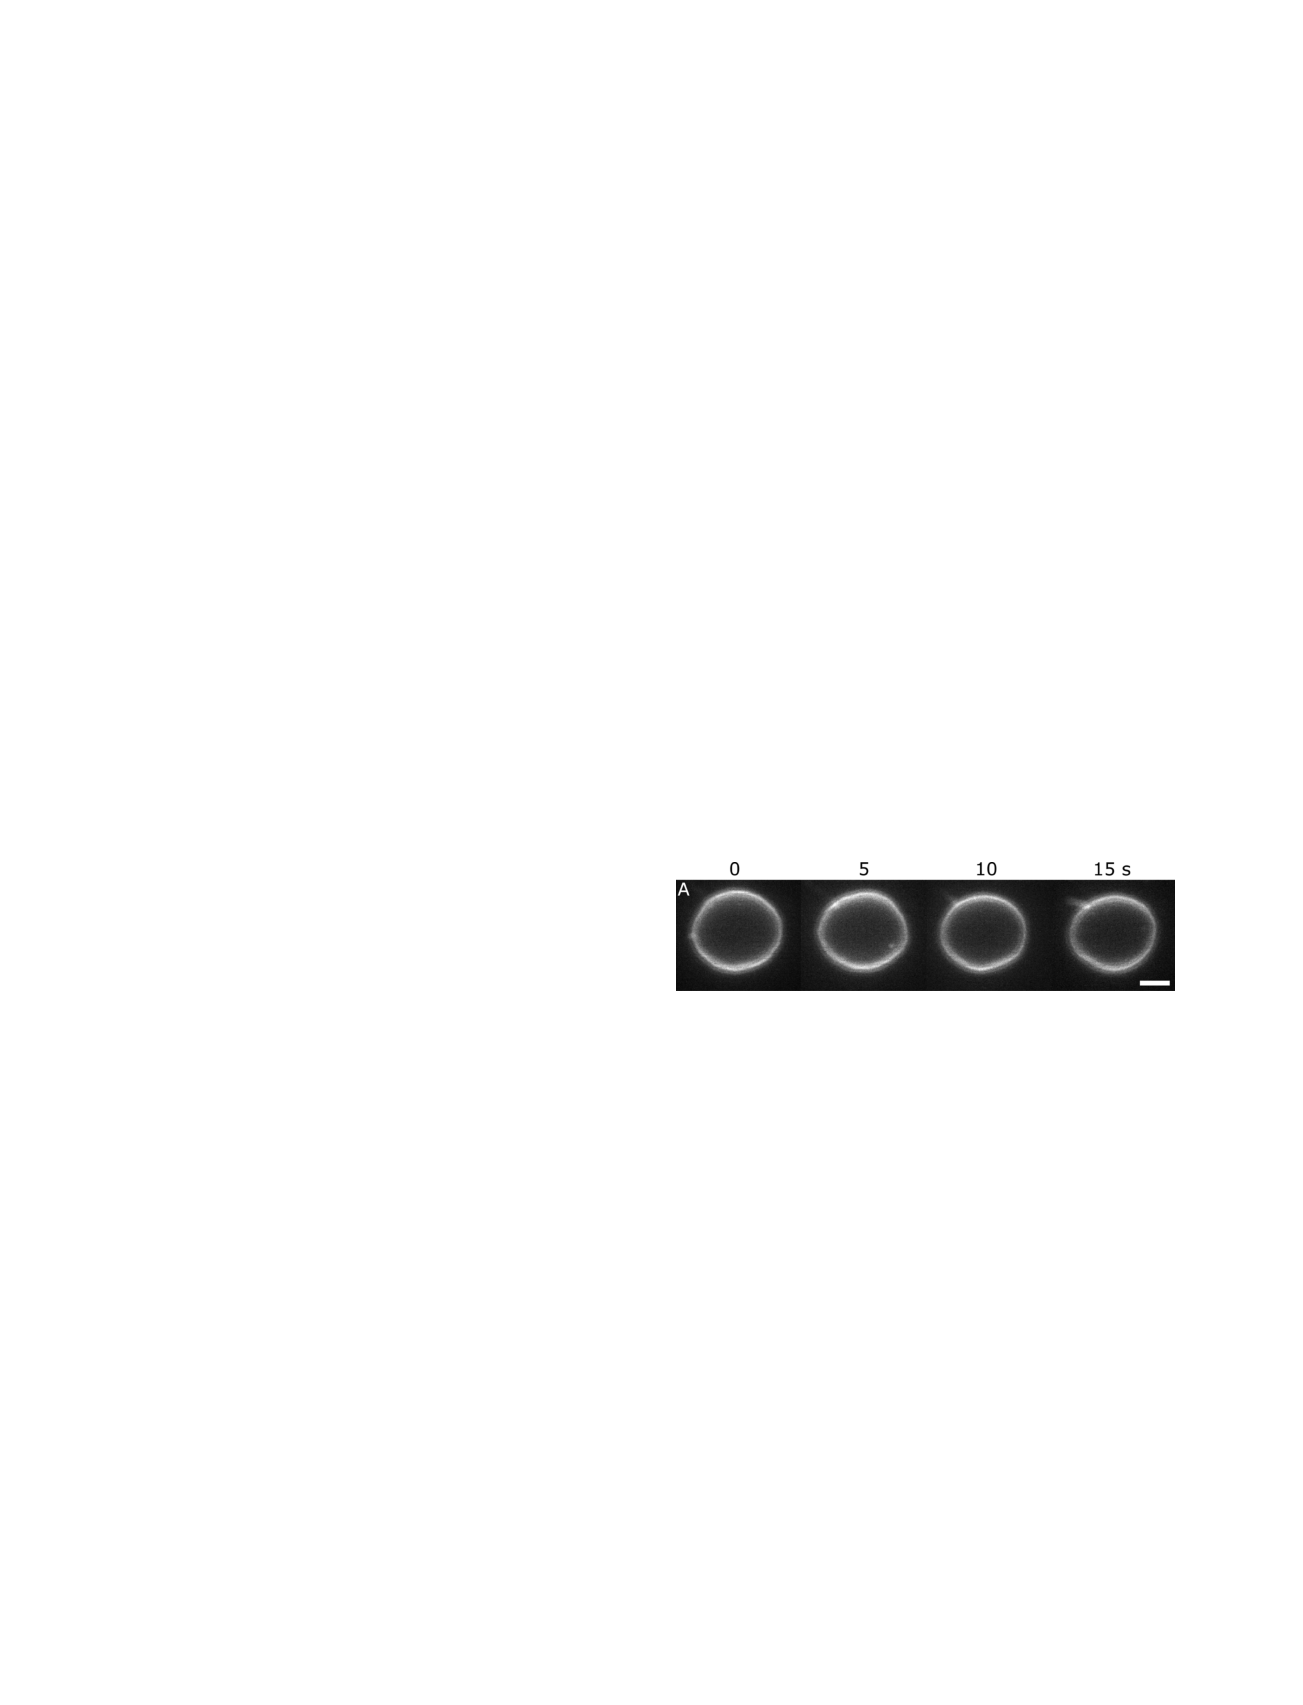
\includegraphics[width=\columnwidth]{\Mempath/Pics/Membrane_fluctuations}
\caption{
مجموعه تصاویر پست سر هم از تغییر شکل یک غشای لیپیدی را با تصویر برداری فلورسانت در بازه‌های ۵ ثانیه‌ای نشان می‌دهد. خط مقیاس سفید رنگ اندازه‌ی ۵ میکرومتر را نشان می‌دهد. 
\cite{ParthasarathyMembraneMeasurement}
}
\label{fig:flucmem}
\end{center}
\end{figure}

مولکول‌های غشا درون یک سیال غوطه‌ور است. مولکول‌ها تحت افت خیز ترمودینامیکی محیط، در جهت‌ درون-صفحه‌ای سطح غشا و جهت عمود بر آن در حال حرکت است. در نتیجه برای تعریف انحنا، لازم است  سطح غشا به بخش‌های کوچک تقسیم بندی شود و با میانگین‌گیری بر روی  مکان مولکول‌ها انحنا را تعیین کرد. اندازه‌ی این بخش‌ها تابع شدت افت و خیز مولکول‌هاست. محاسبات حاصل از  شبیه‌ سازی دینامیک ملکلولی برای غشایی که مولکول‌های یکسان دارد حدود
$5.1$ 
 برابر ضخامت غشا گزارش شده است
\cite{Goetz1998}.
 انحنای هر بخش از یک غشای ساده با ضخامت 
$4nm$,
 حاصل از رفتار دست جمعی حدود 
$100$
مولکول لیپیدی خواهد بود. در مقیاس بزرگ، هر کدام از این بخش‌ها تنها یک نقطه بر روی رویه‌ی غشا را تشکیل می‌دهند. ما می‌توانیم برای هر نقطه روی غشا یک صغحه‌ی مماس و یک صفحه‌ی عمود بر مماس تعریف کنیم. صفحه‌ی عمود بر سطح با رویه‌ی غشا فصل مشترکی به شکل یک خط دارد (مانند شکل 
\ref{fig:normalPlaneIntersection}).
\begin{figure}[h]
\begin{center}
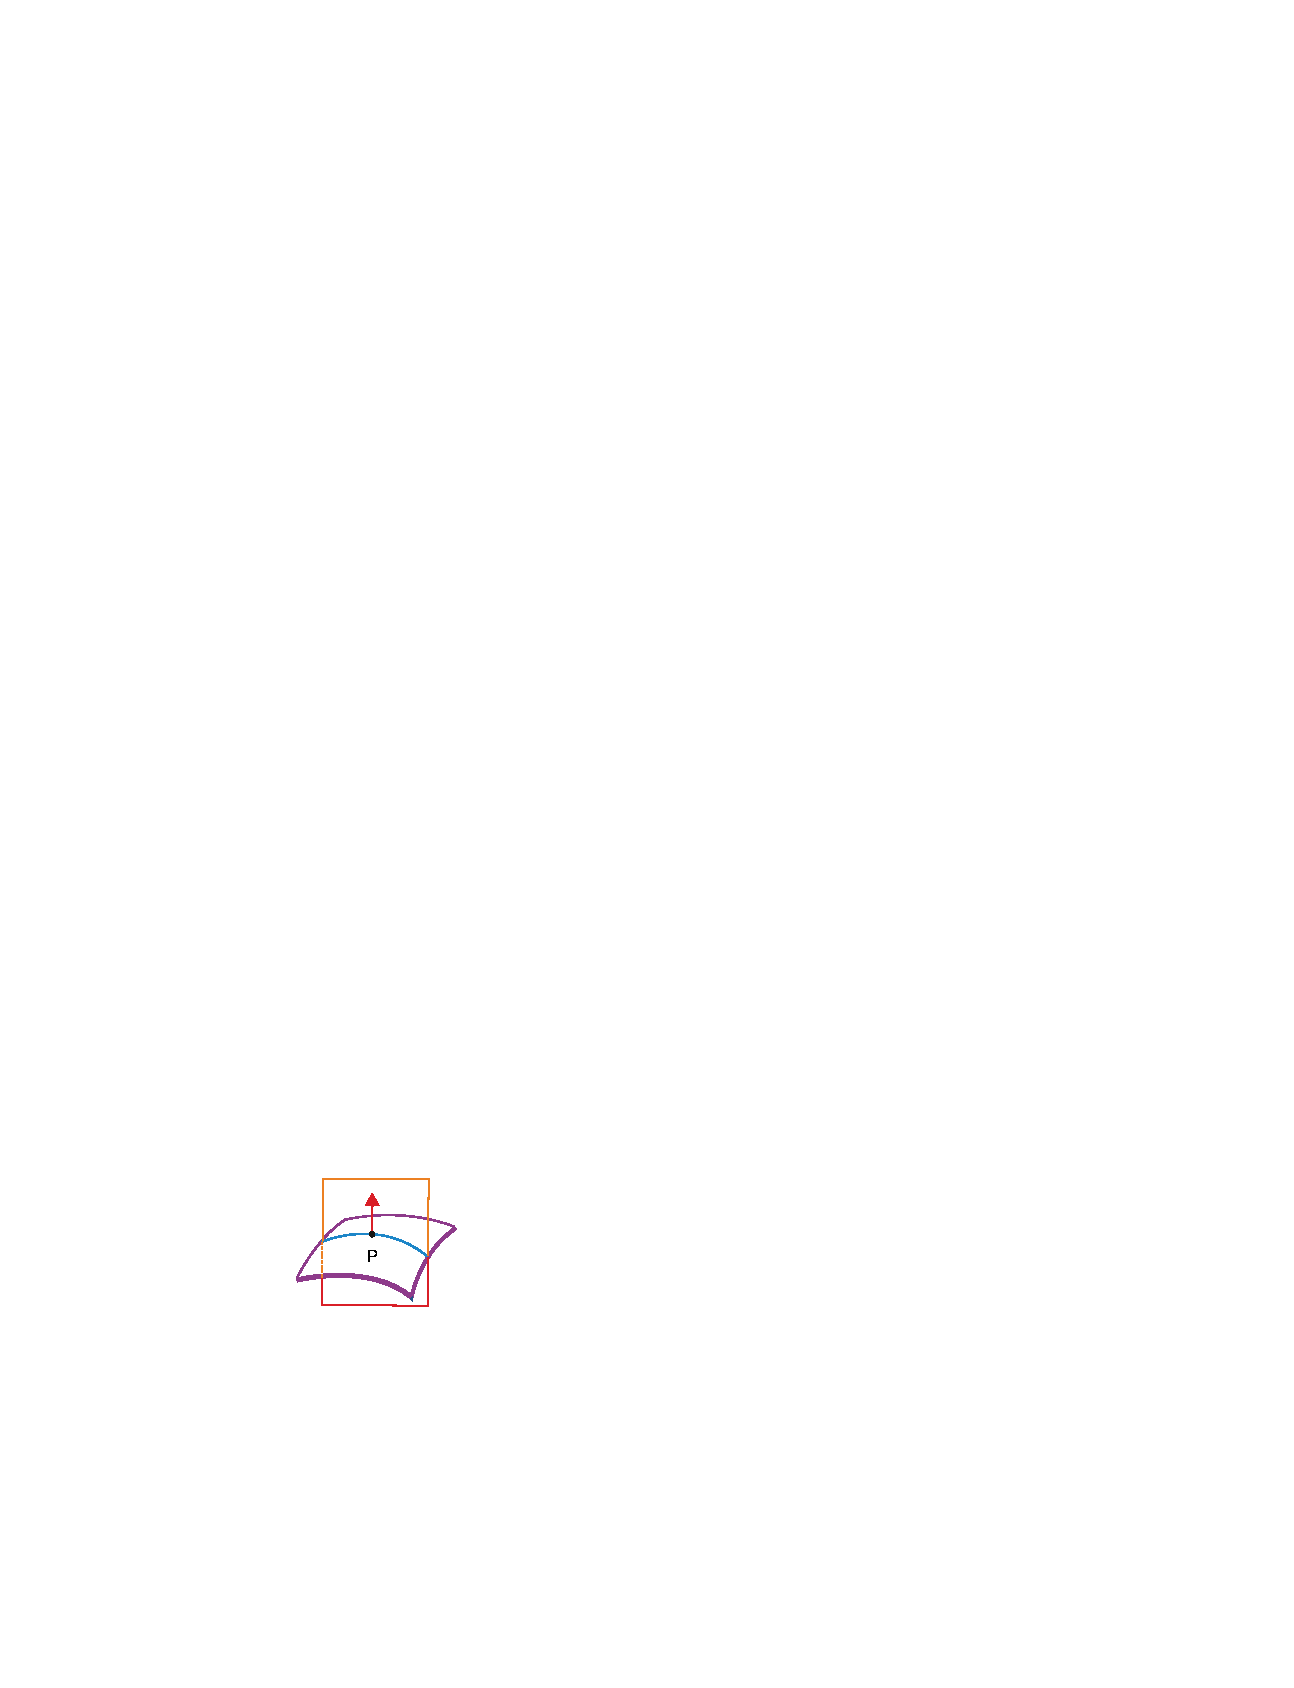
\includegraphics[width=6in]{\MemTB/Pics/NormalPlane}
\caption{
خم حاصل از فصل مشترک صفحه‌ی عمود بر سطح غشا در نقطه‌ی 
P
را نشان می‌دهد.
}
\label{fig:normalPlaneIntersection}
\end{center}
\end{figure}
انحنای تشکیل شده زد فصل مشترک، 
$C$
 در صورتی که در جهت بردار عمود بر سطح باشد 
($\cap$)
 با علامت مثبت و در حالتی که در جهت مخالف باشد 
($\cup$)
 با علامت منفی تعریف می‌شود. می‌توان فرض کرد که خط مشترک قسمتی از یک دایره  است و انحنای این خط عکس شعاع آن دایره خواهد بود. تنها یک  صفحه‌ مماس بر سطح  می‌توان تعریف کرد ولی صفحه‌ی عمود بر سطح می‌تواند در جهت‌های مختلف تعریف شود. انتخاب جهت صفحه‌ی عمود مقدار انحنای محاسبه شده را تغییر خواهد داد. اگر تمام انحناهای ممکن در یک نقطه‌ را با تغییر جهت صفحه‌ی متعامد اندازه‌گیری کنیم، مقادیر در بازه‌ای محدود به  کمینه و بیشینه‌ی انحنا قرار خواهد گرفت،
$C_{min}$
و
$C_{max}$.
 مقادیر کمینه و بیشینه انحنا به انحناهای اصلی سطح معرف هستند که با 
$C_1$
و
$C_2$
نمایش داده می‌شوند. انحناهای اصلی همچنین  ویژه‌مقدار‌های تانسور انحنا در آن نقطه هستند. همچنین اگر انحناهای اصلی برابر یکدیگر نباشند،
$C_1\neq C_2$ 
صفحاتی که خم‌ها با آن تعریف می‌شوند حتما عمود بر هم خواهند بود. از آنجایی که مولکول‌های سطح غشا حرکت پخشی می‌کنند  شکل غشا باید بر اساس تعاریفی باشد که تحت تغییر روش پارامتریزه\LTRfootnote{paprameterisation}  
 کردن سطح ناوردا باشد. انحناهای اصلی سطح چنین ویژگی دارند. انحنای میانگین در هر نقطه‌ بر روی سطح به صورت 
\begin{equation}
M=\frac{1}{2}(C_1+C_2)
\label{eq:meanCurv}
\end{equation}
و انحنای گاووسی به صورت
\begin{equation}
G=C_1C_2
\label{eq:gaussianCurv}
\end{equation}
 تعریف کرد. انحنای میانگین، معادل رَد\LTRfootnote{trace} 
 تانسور انحنا و انحنای گاووسی برابر با دترمینان این تانسور است. همچنین می‌توان روابط بالا را بازنویسی کرد و انحناهای اصلی را بر حسب انحنای میانگین و انحنای گاووسی محاسبه کرد،

\begin{figure}[t]
\begin{center}
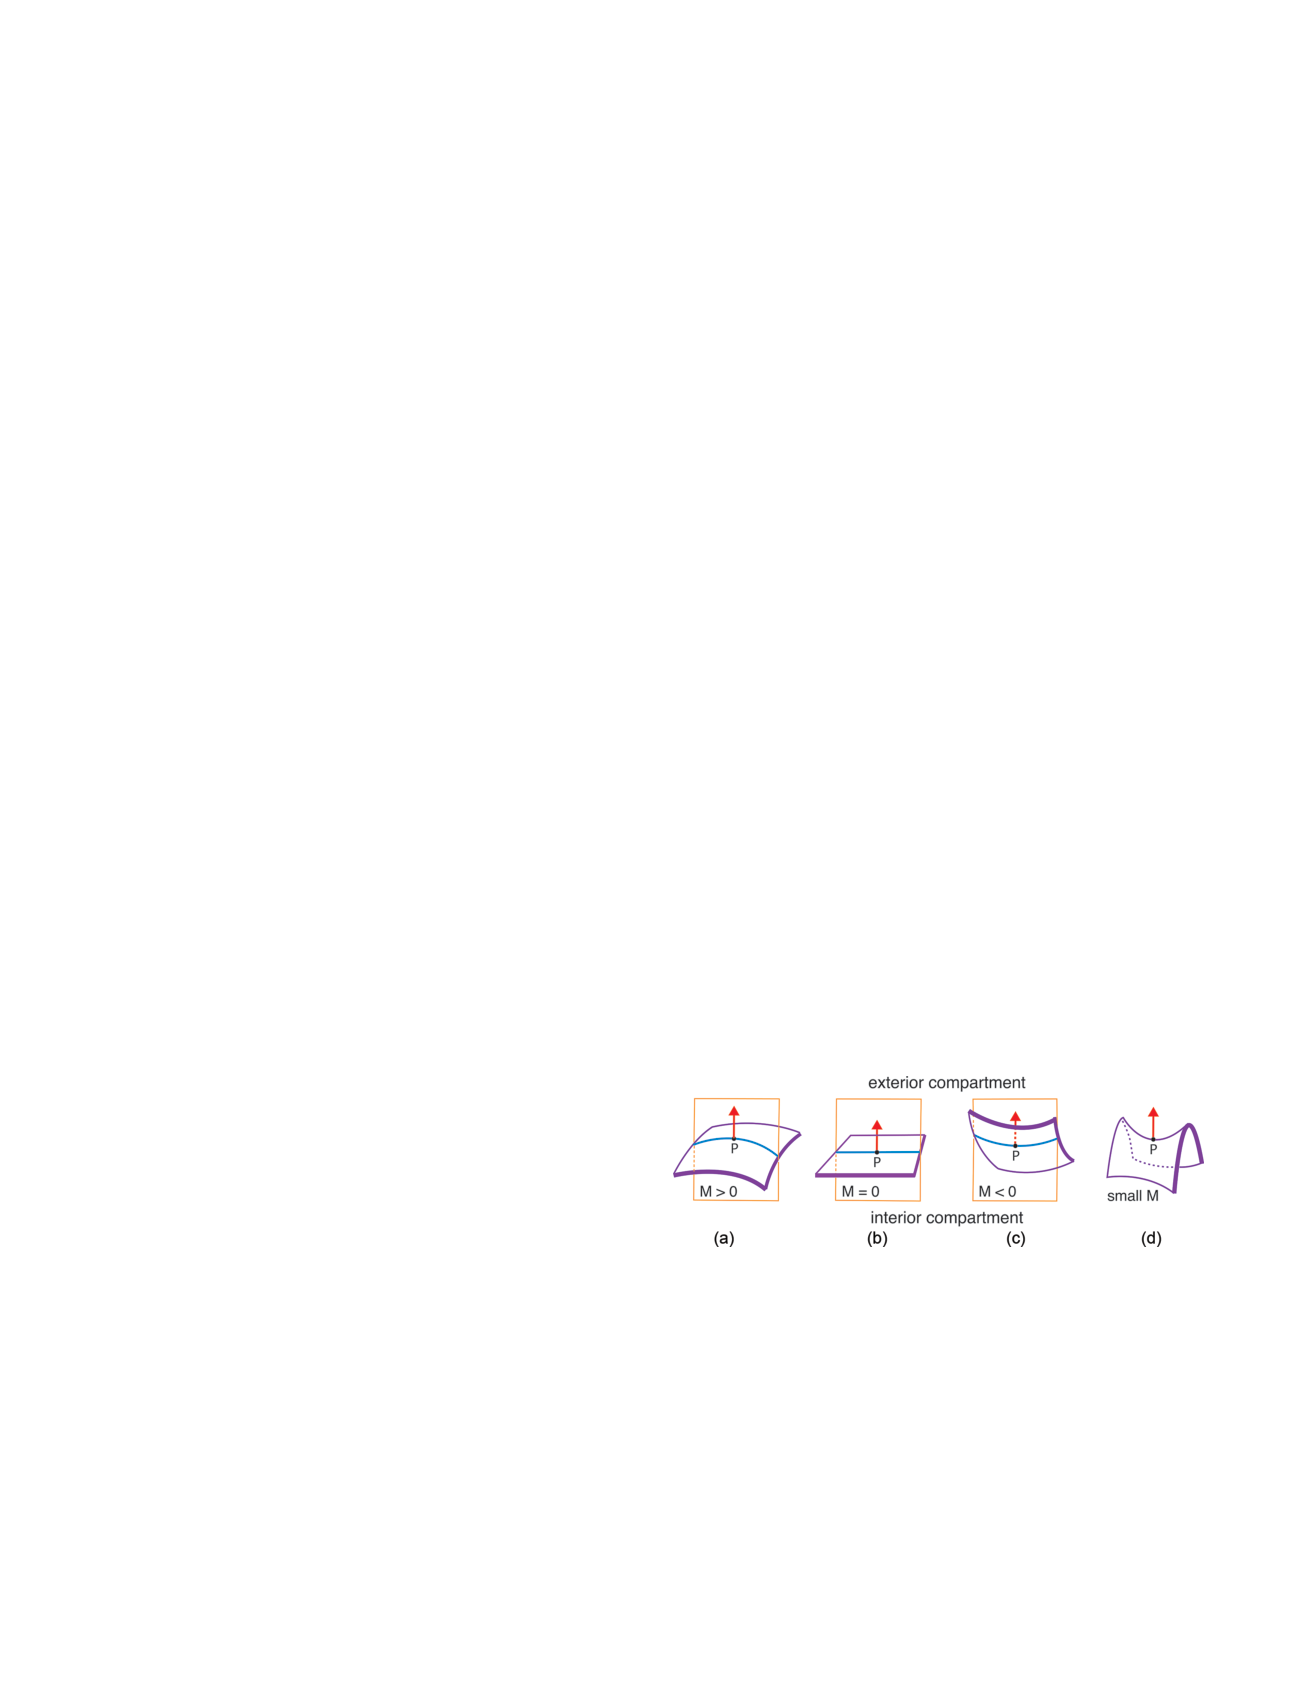
\includegraphics[width=\columnwidth]{\MemTB/Pics/curvatureSign}
\caption{
قرارداد برای تعیین علامت انحنای میانگین. با فرض اینکه بالا محیط خارج غشا و پایین داخل غشا را مشخص کند، بردار نرمال غشا جهت (بردار قرمز رنگ) رو به بالا خواهد داشت. در شکل الف) انحنای میانگین مثبت هنگامی که هر دو انحنای اصلی برآمدگی در جهت بردار نرمال داشته باشند. ب) برای قسمت تخت انحنای میانگین صفر، ج) انحنای منفی هنگامی که  برآمدگی به سمت داخل غشا باشد، د) در نقاط زین اسبی انحناهای اصلی علامت‌های مخالف یکدیگر دارند و در این صورت انحنای میانگین مقدار کمی خواهد داشت.
}
\label{fig:curvatureSign}
\end{center}
\end{figure}

\begin{equation}
\begin{aligned}
C_1&=M-\sqrt{M^2-G}\\
C_2&=M+\sqrt{M^2-G}.
\label{eq:gaussianCurv}
\end{aligned}
\end{equation}
که در روابط بالا، از آنجایی که 
$M^2\geq G$
\cite{Seifert1991}
 هر دو مقدار همیشه حقیقی هستند. مقدار انحنای میانگین، 
 $M$،
 تحت تمامی تبدیل‌های دستگاه مختصات که دترمینان ژاکوبین آن مثبت باشد (جهت بردار عمود بر سطح را تغییر ندهد) تغییر نخواهد کرد. به طور مثال اگر یک سطح با پارامتر‌های 
 $(s^1,s^2)$
 تعریف شده باشد، تبدیلی که پارامتر‌ها را با یکدیگر تعویض کند، 
 $(s^{-1}\equiv s^2,s^{-2}\equiv s^1)$
 تبدیلی است که جهت نرمال سطح را تغییر می‌دهد که در نتیجه علامت انحنای میانگین را تغییر می‌دهد. هرچند که چنین تبدیل‌هایی در فیزیک بسیار مهم هستند زیرا که انتخاب دستگاه مختصات بر مشخصات برخی خواص فیزیکی نباید تاثیرگذار باشد، ولی در مورد انحنا باید تعریف مشخصی برای محاسبات وجود داشته باشد تا بتوان میان محیط داخل و خارج غشا تمییز قائل بشویم. با توجه به رابطه‌ی
 \ref{eq:meanCurv}
 علامت انحنای میانگین در هر نقطه روی غشا تابع مقادیر انحناهای اصلی در آن نقطه‌ است. شکل 
 \ref{fig:curvatureSign}
 حالت‌های مختلف که بر علامت انحنای میانگین تاثیر می‌گذارد را نشان می‌دهد. 

به طور کلی، برای سطح تخت انحنای میانگین صفر است، در صورتی که برآمدگی انحنا به سمت داخل غشا باشد، انحنای میانگین منفی و در صورتی که برآمدگی به سمت بیرون غشا باشد، انحنای میانگین مثبت خواهد بود. در نقاط زین اسبی انحناهای اصلی علامت‌های مخالف یکدیگر دارند و در نتیجه مقدار انحنای میانگین بسیار کوچک خواهد بود. مهم است که اشاره شود که انحنای میانگین ابزار مناسبی برای اندازه‌گیری تاثیر نقاط زین اسبی نیست زیراکه مقدار آن با سطح تخت اختلاف چندانی ندارد. برای اندازه‌گیری تاثیر نقاط زین اسبی، انحنای گاووسی ابزار مناسبی است.
\begin{figure}[t]
\begin{center}
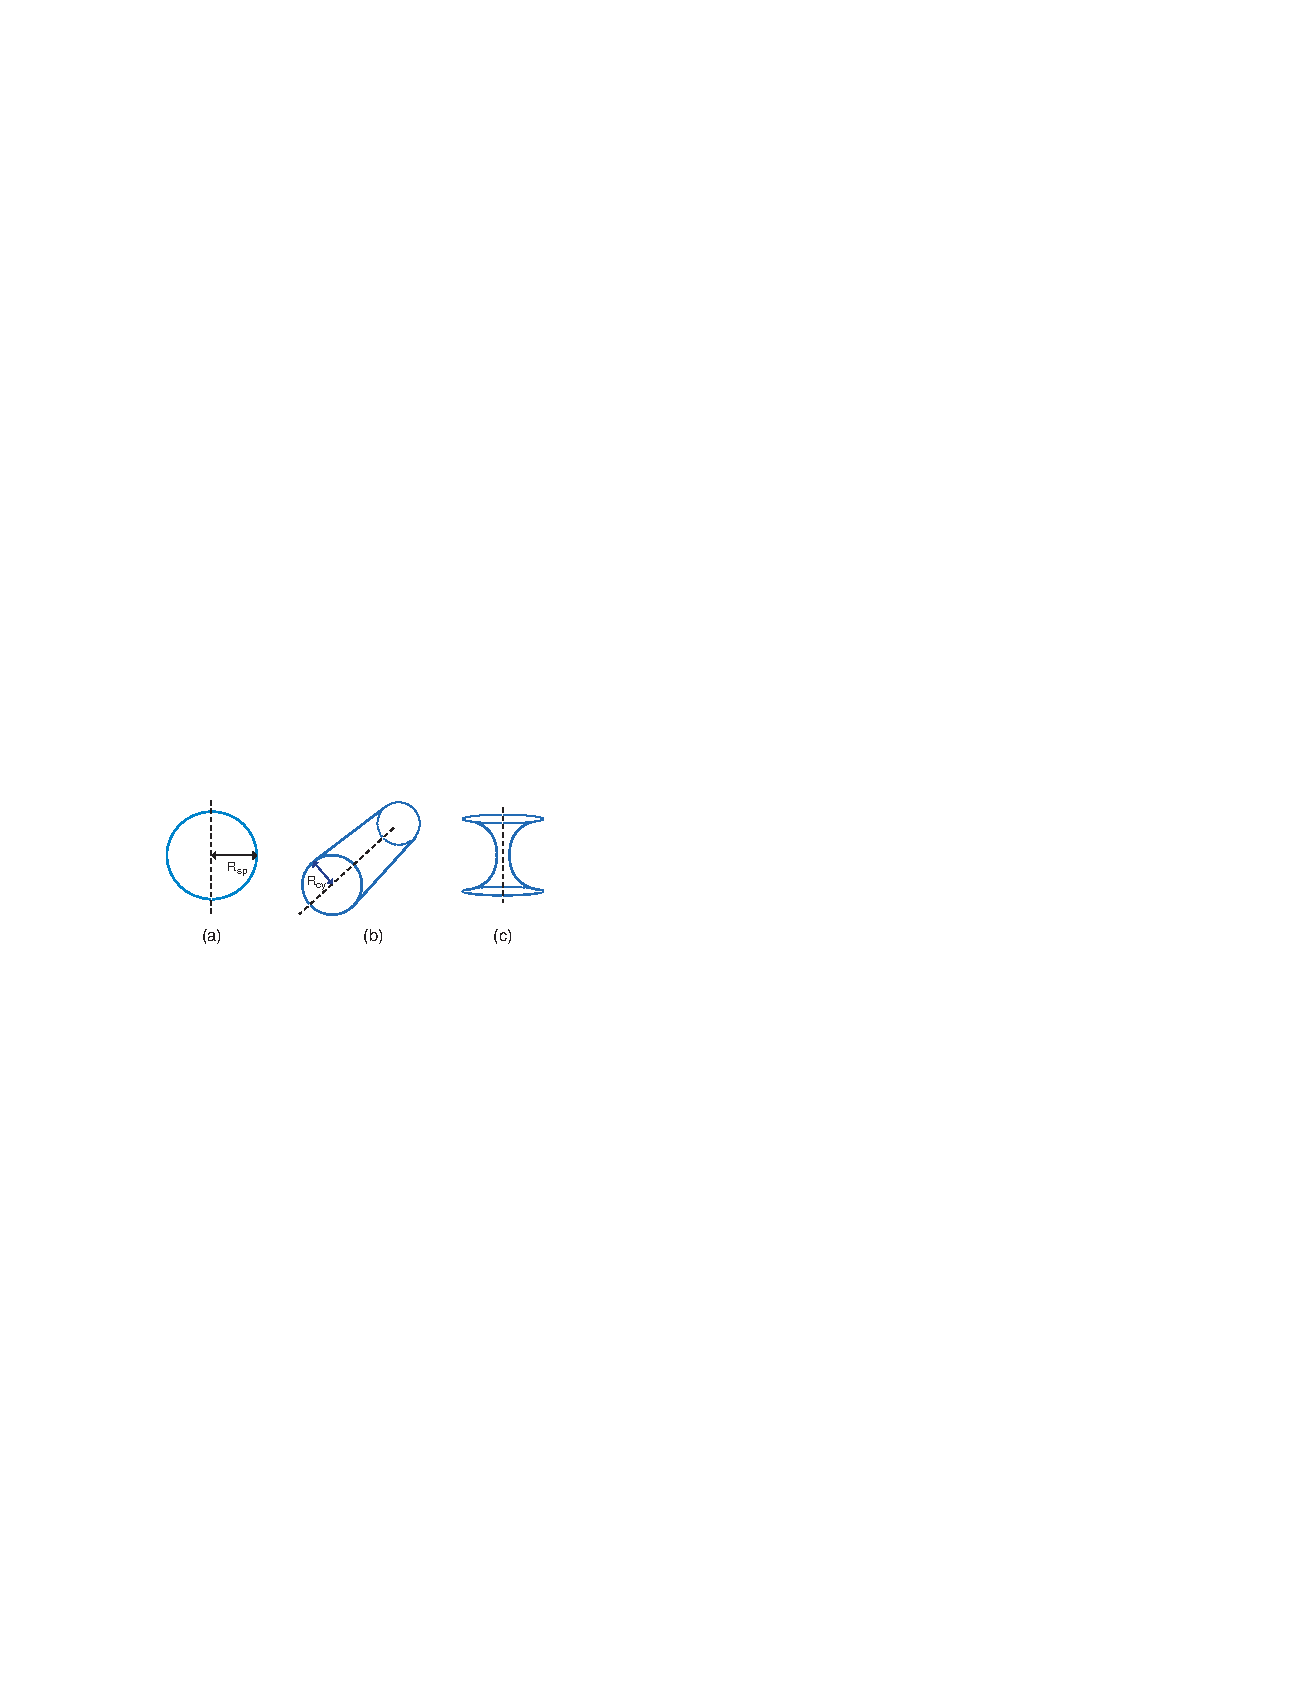
\includegraphics[width=\columnwidth]{\MemTB/Pics/simpleMembraneShapes}
\caption{
شکل‌های ساده‌ی غشا که در تمام نقاط روی سطح انحنای میانگین ثابتی دارند. شکل الف، کُره‌ای به شعاع 
$R_{sp}$
با انحنای میانگین 
$M=\pm 1/R_{sp}$
ب، استوانه‌ای با شعاع 
$R_{cy}$
با انحنای میانگین
$M=\pm 1/2R_{cy}$
و در نهایت ج، کتانوید با انحنای میانگین صفر. علامت انحنای میانگین برای کُره و استوانه به این بستگی دارد که محیط بیرون، سیال خارج از غشا تعریف شود یا سیال داخل.
}
\label{fig:simpleMembraneShapes}
\end{center}
\end{figure}
به طور عمومی انحنای میانگین یک کمیت موضعی است و در نقاط مختلف روی سطح غشا تغییر می‌کند. اما برخی اَشکال ساده در تمامی نقاط روی سطح خود یک مقدار ثابت انحنای میان‌گین دارند. برای مثال انحنای میانگین یک غشای تخت صفر است. برای مثال‌های بیشتر با شکل 
\ref{fig:simpleMembraneShapes}
توجه کنید. انحنای میانگین یک کُره با شعاع
$R_{sp}$
برابر با 
$C=1/R_{sp}$
هنگامی که لایه‌ی خارجی آن با محیط بیرون غشا در ارتباط است و 
$C=-1/R_{sp}$
زمانی که لایه‌ی داخلی آن با محیط بیرون در ارتباط است. همچنین استوانه‌‌ای با شعاع 
$R_{cy}$
دارای انحنای میانگین
$C=\pm1/2R_{cy}$
که علامت آن تابع تعریف جهت بردار عمود خواهد بود. یک شکل ساده‌ی جالب، کتانوید\LTRfootnote{catanoid} 
 است که تمام نقاط روی سطح آن از نقاط زین اسبی تشکیل شده و در نتیجه انحنای میانگین همه جا انحنای میانگین آن صفر است.





 
 
 
 
 




\subsection{
خمش ذاتی
}
تا به اینجا فرض شده که تک لایه‌های تشکیل دهنده‌ی غشا تمایلی به خم شدن در جهت مشخصی ندارند. شکل تعادلی موضعی چنین غشایی یک سطح تخت خواهد بود. کمتر غشایی در طبیعت با چنین تقارنی مشاهده می‌شود ولی دلیل مطالعه‌ی چنین سیستم از نظر مدل‌سازی بسیار پر بهره است چرا که تمام ویژگی‌های الاستیک آن توسط پارامتر سختی خمش
$\kappa$
تعیین می‌شود که مقیاس خوبی برای انرژی یک غشاست. برای غشاهای فسفولیپیدی در دمای اتاق مرتبه‌ی انرژی سختی خمش حدود
$10^{19}J$,
یا
$20k_BT$
است. سختی خمش برای غشاهای از جنس دیگر ممکن است تا حدود یک مرتبه‌ی بزرگی متفاوت باشد. به دلیل اختلاف در ترکیبات تک لایه‌های سازنده‌ی غشاهای زیستی
\cite{Meer2008},
 غشاهای دولایه معمولا نامتقارن هستند. معروف‌ترین مثال غشاهای تشکیل شده از گنگلیوساید 
$GM1$\LTRfootnote{ganglioside GM1}  
است که از نوع گلایکولیپید‌هاست\LTRfootnote{glycolopids}  
و در غشاهای سلول‌های عصبی پستانداران به طور فراوان یافت می‌شود. 
$GM1$
نقش لنگر را برای مواد سمی، باکتری‌ها، و ویروس‌ها بازی می‌کند
\cite{Ewers2010}.
نحوه‌ی تغییر خمش موضعی با تغییر غلظت 
$GM1$
به طور مفصل به شکل تجربی
\cite{Bhatia2018, Raktim2018}
و هم به شکل شبیه‌سازی
\cite{Raktim2018, Sreekumari2018}
مطالعه شده‌است. همچنین جهت‌گیری پروتئین‌های درون غشا، چسبیدن پروتئین‌های محیط بر سطح غشا معمولا خمش را تغییر می‌دهد. در نتیجه اگر ذرات زیادی به سطح غشا بچسبند، خمش ذاتی در سطح غشا،
$C_0$
، ایجاد خواهد شد
\cite{Lipowsky2002}
که تابع تعداد ذراتی‌ است که به تک‌لایه‌های مختلف غشا متصل شده باشند
\cite{Breidenich2000}.
 مقدار خمش ذاتی بسیار متغییر است و از مقیاس موضعی 
$1/10nm$
تا مقیاس خود غشا
$1/50\mu m$
گزارش شده است.


\subsection{
نظریه‌ی مدل خمش ذاتی
\label{sec:spontaneousCurvatureModel}
}
در این بخش به بنا کردن چهارچوب نظریه‌ای پرداخته می‌شود که نقش کلیدی در فهم شکل‌های غشا‌های غول‌آسا داشته است. این نظریه بر اساس انرژی الاستیک خمش غشا ایجاد شده‌است. همچنین در این نظریه حل‌شوندگی بسیار کم مولکول‌های لیپیدی و تاثیر اختلاف فشار اسمزی به شکل قید روی سطح و حجم غشا در نظر گرفته شده است. درواقع جذابیت این نظریه در توصیف تبادل بین انرژی‌هایی است با منشا موضعی و سراسری. از طرفی شکل انحنای غشا بر اساس انرژی‌های ناشی از خمش‌های موضعی (خمش میانگین و خمش گاووسی) تعیین می‌شود و از طرف دیگر با فرض اینکه غشا تغییر توپولوژیکی نداشته باشد (با غشای دیگری جوش نخورد، تکه‌ای از غشا به شکل جوانه از آن جدا نشود، یا حفره‌ای در آن ایجاد نشود) سطح و حجم ثابتی خواهد داشت که بر شکل نهایی که غشا می‌تواند به خود بگیرد تاثیر بسیار مشخصی دارد. ارتباط میان پدیده‌های موضعی و سراسری با دو کمیت به نام تنش مکانیکی\LTRfootnote{mechanical tension}  
$\gamma_{ten}$
و اختلاف فشار
$\Delta P$
برقرار می‌شود.

نظریه‌ی مدل خمش ذاتی\LTRfootnote{spontaneous curvature model}  
یک غشا را با دو مشخصه‌ی هندسی، سطح غشا 
$A$
و حجم آن 
$V$
، به همراه دو مشخصه‌ی مادی\LTRfootnote{material property}  
سختی خمش غشا
$\kappa$
و خمش ذاتی 
$C_0$
آن توصیف می‌کند. مدل خمش ذاتی بر اساس انرژی خمش بر حسب توان‌های خمش‌های اصلی پایه‌گزاری شده و تا زمانی که خمش نسبت به عکس ضخامت غشا کوچک باشند پابرجاست.
انرژی انحنای غشایی که شکل 
$S$
را دارد 
$\mathcal{E}_{cu}\{S\}$
است که بر حسب انتگرال سطحی چگالی موضعی انرژی 
$\varepsilon_{cu}(S)$
تعریف می‌شود،
\begin{equation}
\mathcal{E}_{cu}\{S\}=\int dA~\varepsilon_{cu}(S).
\end{equation}
فرض می‌کنیم چگالی انرژی موضعی تنها تابع خمش‌های اصلی 
$C_1$
و
$C_2$
است. همچنین اگر در هر نقطه بر روی سطح غشا دستگاه مختصات را 
$\pi/2$
در جهات بردار عمود برسطح دوارن دهیم، انرژی خمش نباید تغییر کند،
$\varepsilon_{cu}(C_1,C_2)=\varepsilon_{cu}(C_2,C_1)$.
بسط انرژی تا جمله‌ی توان دوم به شکل حدی با معادله‌ی زیر برابر خواهد بود،
\begin{equation}
\varepsilon_{cu}(C_1,C_2)\approx a_0+a_1(C_1+C_2)+a_2(C_1^2+C_2^2) + a_3 C_1C2.
\end{equation}
این بسط را می‌توان بر حسب خمش میانگین و خمش ذاتی به شکل زیر باز نویسی کرد،
\begin{equation}
\varepsilon_{cu}\approx 2\kappa(M-C_0)^2+\kappa_GG.
\end{equation}
با جایگذاری در انتگرال سطحی شکل انرژی انحنای هلفریش
\LTRfootnote{Helfrich}
\cite{Helfrich1973}
بدست می‌آید،
\begin{equation}
E_{cu}=\int dA\left[\frac{1}{2}\kappa(C_1+C_2-2C_0)^2+\kappa_GC_1C_2\right],
\label{eq:HelfrichCurvatureEnergy}
\end{equation}
که به دو انتگرال انرژی خمش 
\begin{equation}
E_{b}=\frac{1}{2}\kappa\int dA (C_1+C_2-2C_0)^2
\label{eq:HelfrichBendingEnergy}
\end{equation}
و انرژی خمش گاووسی
\begin{equation}
E_{G}=\kappa_G\int dA C_1C_2
\label{eq:HelfrichGaussianEnergy}
\end{equation}
تقسیم می‌شود.
در صورتی که غشا هندسه‌ی بسته داشته باشد و هیچ لبه‌ی آزادی در آن نباشد (مثلا یک شکل کُروی داشته باشد و به شکل یک صفحه‌ی آزاد در محیط نباشد) قضیه‌ی گاووس-بونت\LTRfootnote{Gauss-Bonnet theorem}
\cite{NelsonBook2004}
در هندسه‌ی دیفرانیسیلی جواب انتگرال معادله‌ی
\ref{eq:HelfrichGaussianEnergy}
 تابع مشخصه‌ی اویلری رویه\LTRfootnote{Euler characteristic of the surface}
 یا جینوس\LTRfootnote{genus}
خواهد بود.
 \begin{equation}
E_{G}=\kappa_G\int dA C_1C_2=2\pi\kappa_G(2-2g).
\label{eq:GaussianBonnet}
\end{equation}
 
 جینوس سطح تعداد سوراخ‌هایا تعداد دسته‌های یک شکل را می‌شمارد.
مثلا یک کُره هیچ سوراخ یا دسته‌ای ندارد و جینوس آن صفر است. در صورتی که یک شکل چنبره\LTRfootnote{toroid}
یک سوراخ یا دسته دارد و جینوس آن یک است
$g=1$
. همچنین رویه‌ای که سطح یک لیوان دسته‌دار را می‌پوشاند جینوس برابر با یک خواهد داشت (به مثال‌های شکل 
\ref{fig:genus012}
توجه کنید).
\begin{figure}[t]
\begin{center}
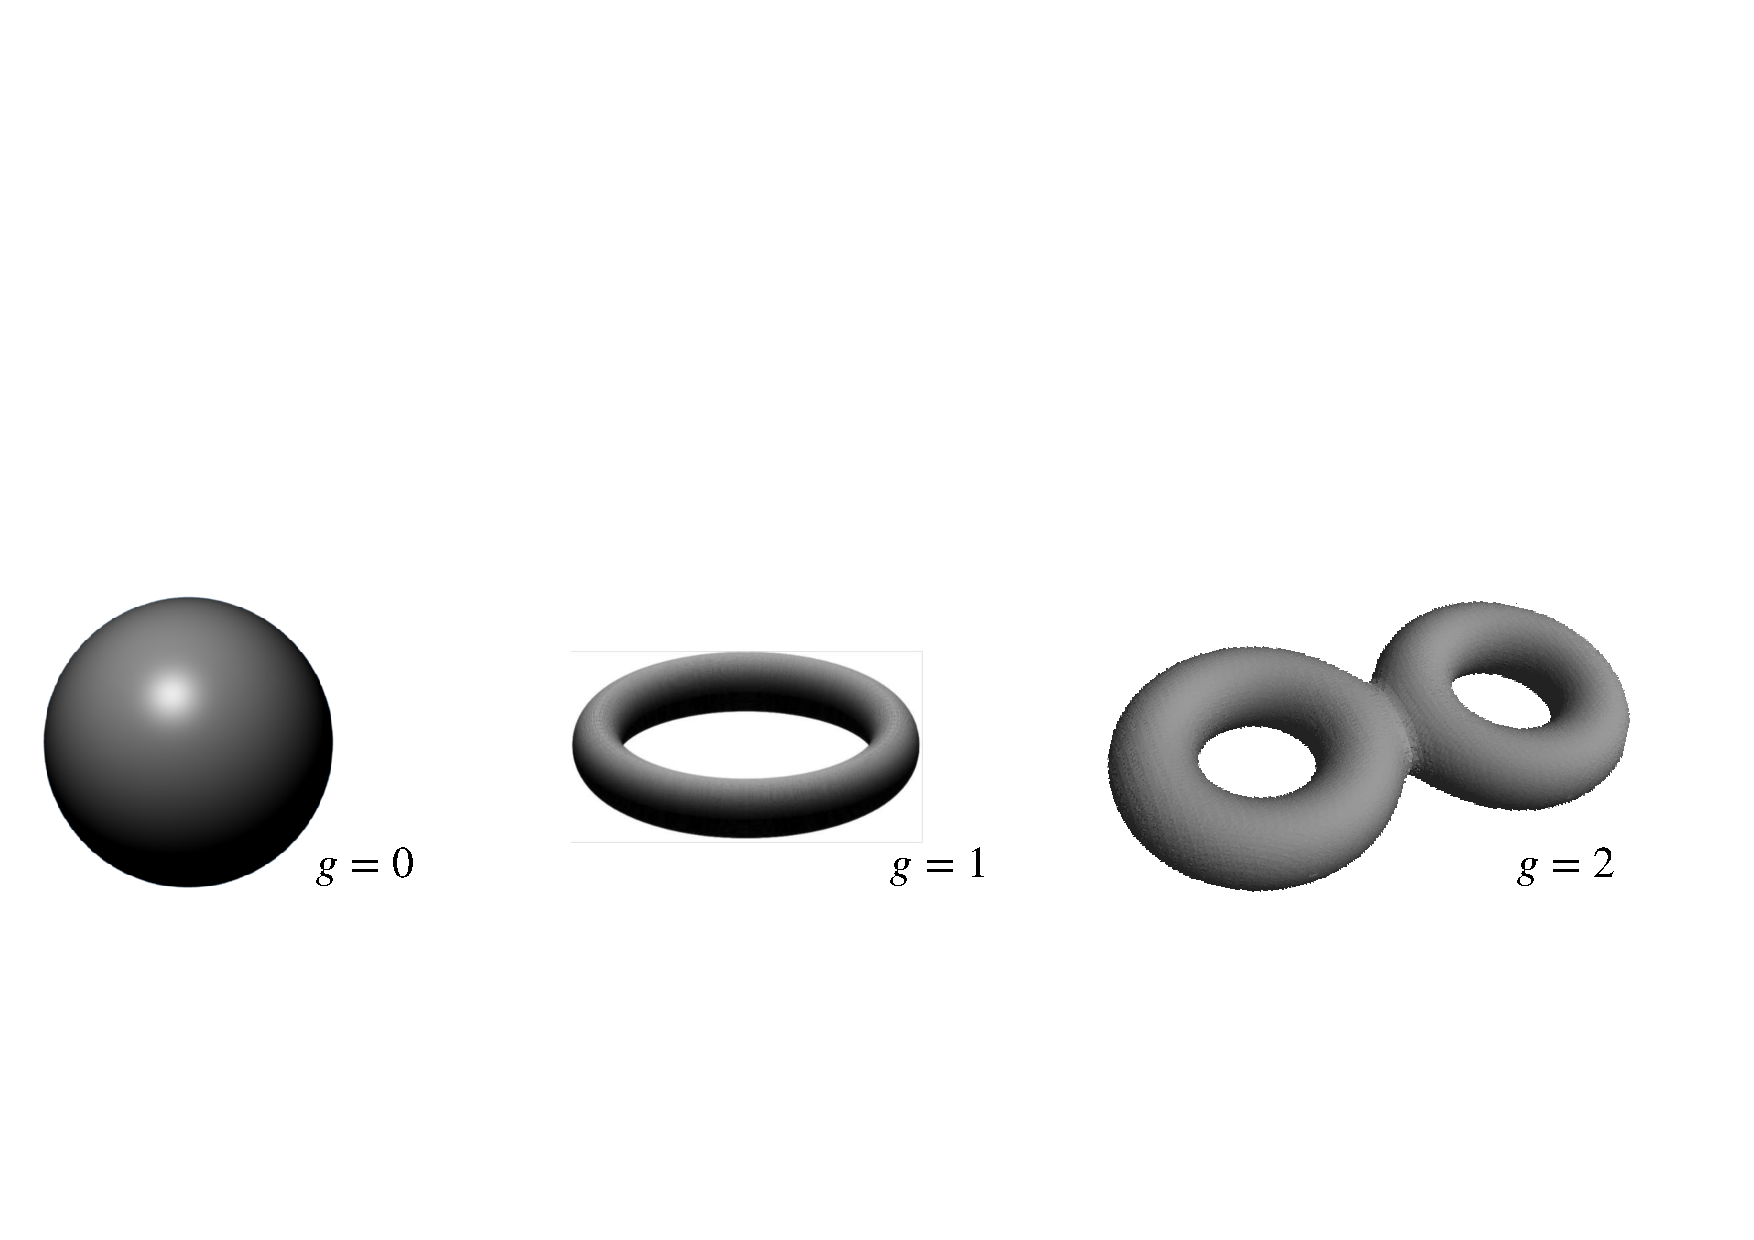
\includegraphics[width=\columnwidth]{\MemTB/Pics/genus}
\caption{
به ترتیب از چپ به راست یک کُره، چنبره، و دو چنبره متصل به هم را مشاهده می‌کند که به ترتیب شکلی با 
$0$, $1$,
 و 
$2$
سوراخ/دسته که همچنین مقدار جینوس این سطوح را تعیین می‌کند.
}
\label{fig:genus012}
\end{center}
\end{figure}
برای مثال انرژی انحنای یک کُره به شعاع
$R$
را با استفاده از معادلات
\ref{eq:HelfrichBendingEnergy}
و
\ref{eq:HelfrichGaussianEnergy}
محاسبه می‌کنیم. با فرض اینکه بردار عمود بر سطح کره در جهت خارج کُره تعریف شده باشد، از انجایی که شعاع‌ کره در تمام نقاط سطح آن ثابت است خمش در سراسر سطح با یک مقدار
$C_1=C_2=1/R$
تعیین می‌شود. تنها فرض باقی مانده تعیین خمش ذاتی شکل است. در صورتی که فرض شود حالت تعادلی رویه‌ای که کُره را تشکیل داده سطح تخت باشد
$C_0=0$
انرژی آن
 \begin{equation}
 \begin{aligned}
E_{b}&=\frac{1}{2}\kappa\int R^2d\Omega (\frac{2}{R}-0)^2=8\pi\kappa\\
E_{G}&=\kappa_G\int R^2d\Omega \frac{1}{R^2}=4\pi\kappa_G=2\pi\kappa_G(2-2g)=2\pi\kappa_G(2-0) \\
E_{cu}&=8\pi\kappa+4\pi\kappa_G.
\end{aligned}
\end{equation}
در صورتی که خمش ذاتی آن،
$C_0=1/R$
باشد انرژی انحنای آن
 \begin{equation}
 \begin{aligned}
E_{b}&=\frac{1}{2}\kappa\int R^2d\Omega (\frac{2}{R}-\frac{2}{R})^2=0\\
E_{G}&=2\pi\kappa_G(2-2g)=4\pi\kappa_G \\
E_{cu}&=4\pi\kappa_G
\end{aligned}
\end{equation}
است. توجه کنید که انرژی انحنای محاسبه شده تابع شعاع کُره نیست. به طور عمومی انرژی محاسبه شده با مدل خمش ذاتی از مقیاس شکل مستقل است. در نتیجه مدول خمشی
$\kappa$
نیز تابع مقیاس سیستم نخواهد بود. این مفهوم بسیار متفاوت از تعاریف رایج از مدول خمشی برای پلیمر‌هاست و باید توجه ویژه‌ای به این نکته بشود. از آنجایی که در مطالعه‌ی شکل غشا معمولا اختلاف انرژی بین اشکال اهمیت دارد و (به خصوص برای محاسبه‌ی نیرو) تا زمانی که غشا تغییر توپولوژیکی نداشته باشد، از محاسبه‌ی مقدار ثابت انرژی خمش گاووسی چشم پوشی می‌شود. 





































\subsection{
حجم کاهیده
}
همانطور که در فصل اول توضیح داده شد. غشاهای زیستی نمیه‌تراوا هستند. یعنی حجم آب درون آنها توسط دمای محیط، غلظت ملکول‌های محیط، و ملکول‌های درون آن یا به طور عمومی شرایط اسمزی محیط مشخص می‌شود. در صورتی که اختلاف فشار اسمزی از بیرون بالا باشد، غشا ممکن است مچاله شود، بر روی خود تا شود، و یا غشا‌های کچک‌تری تشکیل دهد. ملکول‌های لیپید بسته به شرایط محیطی (مثلا دما) با چیدمان مشخصی فضا را اشغال می‌کنند. با فرض اینکه تعداد ملکول‌های غشا تغییر نکند، سطح غشا در طول عمر آن ثابت خواهد بود. از طرفی تحت اختلاف فشار اسمزی منفی، غشا متورم خواهد شد. البته میزان تغییر سطح غشا فقط در حدود چند درصد است و در صورتی که نیاز به تغییر سطح بیشتری باشد، پاره خواهد شد. برای غشایی با مساحت
$A$
شعاع کُره‌ای معادل که همان مساحت را داشته باشد،
\begin{equation}
R_{ve}=\sqrt{\frac{A}{4\pi}}
\end{equation}
است. از آنجایی که بیشترین حجمی که غشا می‌تواند داشته باشد حجم یک کُره‌ است، حجم غشا همیشه کمتر مساوی این مقدار خواهد بود،
\begin{equation}
V\leq\frac{4\pi}{3}R_{ve}^3=\frac{4\pi}{3}\left(\frac{A}{4\pi}\right)^{\frac{3}{2}}
\end{equation}
در نتیجه می‌توان حجم کاهیده به شکل زیر تعریف کرد،
\begin{equation}
\nu=\frac{V}{\frac{4\pi}{3}R_{ve}^3}=6\sqrt{\pi}VA^{-\frac{3}{2}}
\label{eq:reducedVolume}
\end{equation}
که همیشه کوچک‌تر از یک است و در صورتی که غشا شکل کُره‌ای بی نقص داشته باشد برابر یک خواهد بود.

\subsection{
تنش 
}
در حالت تعادلی، مولکول‌های لیپیدی، با توجه به شرایط ترمودینامیکی محیط، سطح غشا را با چیدمانی بهینه‌ می‌پوشانند.  به علت وجود نیروهای خارجی یا قیود مختلف،  سطح غشا از سطح تعادلی
$A_0$
تغییر کرده، و در سطح غشا تنش  
$\gamma_{st}(A)$
ایجاد خواهد شد. از آنجایی که غشا ماهیت سیال‌گون دارد،  تنشی که حاصل آن تنها جابجایی مولکول‌ها روی سطح باشد (تنش برشی\LTRfootnote{shear})
 انرژی سطح را تغییر نخواهد داد. تنها تنشی که مساحت کل غشا را تغییر دهد با مقاومت روبرو خواهد شد. تنش غشا تا مرتبه‌ی اول در جمله‌ی 
$(A-A_0)$
به شکل زیر تعریف می‌شود،
\begin{equation}
\gamma_{st}(A)=k_A\frac{A-A_0}{A_0}.
\end{equation}
در این معادله
$k_A$
مدول فشردگی سطحی\LTRfootnote{area compressibility modulus}
است
\cite{thegiantvesiclebook2019}.
 بدیهی‌است که این رابطه تا زمانی که تنش ایجاد شده از  آستانه‌ی پاره شدن غشا کمتر باشد قابل استفاده است. برای غشاهای لیپیدی، آستانه‌ی پاره شدن دو مرتبه‌ی بزرگی کوچک‌تر از مدول فشردگی سطحی و حدود چند
$mN/m$
است. انرژی تنش ایجاد شده حاصل از تغییر مساحت غشا، معادل کار انجام شده برای تغییر سطح است،
\begin{equation}
E_{st}(A)=\int_{A_0}^A dA~\gamma_{st}(A)=\frac{1}{2}k_A\frac{(A-A_0)^2}{A_0}.
\label{eq:surfaceTension}
\end{equation}
مشابه به این بحث می‌توان هزینه‌ی انرژی برای تغییر حجم سیال درون غشا را نیز به صورت زیر تعریف کرد
\cite{discher1998biophysicaljournal},
\begin{equation}
E_{v}(V)=\frac{1}{2}k_V\frac{(V-V_0)^2}{V_0}.
\label{eq:volumeEnergy}
\end{equation}
  در اینجا
$k_V$
مدول فشردگی حجمی\LTRfootnote{volume compressibility modulus}
 و 
$V_0$
حجم تعادلی سیال درون غشا است.









\section{
انرژی کشش الاستیک
}
%\setRL
%\pagenumbering{arabic} 

بعضی غشاها تنها از یک غشای دو‌-لایه‌ی لیپیدی تشکیل نشده‌اند. مانند غشای هسته‌ی سلول‌های پستانداران که معمولا از دو غشای لیپیدی دو لایه متصل به یک شبکه‌ی پلیمری دو بعدی الاستیک تشکیل شده‌است. در این بخش به مدل‌سازی انرژی شبکه‌های پلیمری الاستیک می‌پردازیم.
%\subsection{
%انرژی کشش در سطح
%}
اگر فرض کنیم جابجایی روی یک عنصر سطحی حاصل از کشیده‌ یا فشرده شدن سطح با بردار 
$u$
توصیف شود، با فرض خطی بودن عکس العمل ماده، انرژی پتانسیل حاصل از تغییر شکل سطح را می‌توان با معادله‌ی زیر بررسی کنیم،
\begin{equation}
E_{stretching}=\frac{1}{2}Y_{2D}A\varepsilon^2.
\end{equation}
که اینجا 
$Y_2D$
مدول دو بعدی یانگ،
$A$
سطح عنصر در حالت کشیده نشده، و
$\varepsilon$
تانسور کرنش است. تانسور کرنش برای سطح دو بعدی به شکل زیر تعریف می‌شود:
\begin{equation}
\varepsilon_{ij} = \frac{1}{2}(u_{ij}+u_{ji})
\end{equation}


در نظریه‌ی الاستیک سطح هر تغییر شکل با یک میدان بردار جابجایی 
$u(r)=(u_1,u_2)$
نشان داده می‌شود نقطه‌ی 
$r(x,y)$
را به نقطه‌ی 
$r+u$
نگاشت می‌کند. اگر در شبکه نقص وجود نداشته باشد این نگاشت یک به یک خواهد بود. در صورتی که فرض کنیم که ماده مورد مطالعه یکنواخت و همسانگرد است، برای جابجایی‌های کوچک (رژیم خطی) قانون هوک را به شکل توان دوم تانسور کرنش\LTRfootnote{Cauchy, 1822; Lam ́e, 1852}
نوشت،
\begin{equation}
E_s=\frac{1}{2}\int d^2r(2\mu u_{ij}^2+\lambda u_{kk}^2).
\label{eq:energylame}
\end{equation}
در اینجا $\lambda$
و $\mu$
ثابت‌های لم\LTRfootnote{Lamé Coefficients}
است. ما می‌دانیم که تانسور کرنش به شکل زیر تعریف می‌شود،
\begin{equation}
u_{ij}=\frac{1}{2}(\partial_i u_j+\partial_j u_i+\partial_i u_k\partial_j u_k).
\end{equation}
اما برای جابجایی کوچک از جمله‌ی غیر خطی صرف نظر می‌کنیم و تانسور کرنش را به این شکل تعریف می‌کنیم،
\begin{equation}
u_{ij}=\frac{1}{2}(\partial_i u_j+\partial_j u_i).
\label{eq:simplestrain}
\end{equation}
می‌توانیم  از انرژی کششی گرادیان بگیریم و مقدار کمینه‌ی آن را بررسی کنیم، در نتیجه،
\begin{equation}
\begin{aligned}
&\partial_i\sigma_{ij}=0\\
&\sigma_{ij}=2\mu u_{ij}+\lambda u_{kk}\delta_{ij}.
\label{eq:stress}
\end{aligned}
\end{equation}
در این معادله 
$\sigma_{ij}$
تانسور تنش است. معادله‌ی 
\ref{eq:stress}
را به تنهایی می‌توان حل کرد ولی از آنجایی که دیورژانس تنش صفر است معمول است که این معادله را به شکل یک پتانسیل اسکالر بنویسیم،
\begin{equation}
\sigma_{xx}=\frac{\partial^2\chi}{\partial y^2},\quad\sigma_{yy}=\frac{\partial^2\chi}{\partial x^2},\quad\sigma_{xy}=\frac{\partial^2\chi}{\partial_x\partial_y}.
\end{equation}
انتخاب‌های خیلی زیادی می‌توانند معادله‌ی بالا را ارضاء خواهد کرد، ولی جواب‌هایی که به لحاظ فیزیک قابل قبول هستند باید بتوانند رابطه‌ی بین میدان جابجایی و 
$\chi$
را رعایت کنند،
\begin{equation}
\begin{aligned}
\frac{1}{2}(\partial_iu_j+\partial_ju_i)&=u_{ij}\\
&=\frac{1+\nu}{Y}\sigma_{ij}-\frac{\nu}{Y}\sigma_{ll}\sigma_{ij}\\
&=\frac{1+\nu}{Y}\epsilon_{im}\epsilon_{jn}\partial_{m}\partial_{n}\chi-\frac{\nu}{Y}\nabla^2\chi\delta_{ij}.
\label{eq:constraint}
\end{aligned}
\end{equation}
در اینجا $Y$
و $\nu$
به ترتیب مدول ۲ بعدی یانگ\LTRfootnote{2D Young Modulus}
 و نسبت پواسون\LTRfootnote{Poisson ratio}
است که بر حسب ضرایب لم به شکل زیر بیان می‌شوند،
\begin{equation}
\begin{aligned}
Y&=\frac{4\mu(\mu+\lambda)}{2\mu+\lambda}\\
\nu&=\frac{\lambda}{2\mu+\lambda}.
\label{eq:younglame}
\end{aligned}
\end{equation}

 
 
 
 
 
 











